\documentclass{standalone}
\usepackage[utf8]{inputenc}
\usepackage[T1]{fontenc}
\usepackage{graphicx}
\usepackage{amsmath}
\usepackage[american,siunitx]{circuitikz}
\usetikzlibrary{arrows,shapes,calc,positioning}

    
\begin{document}
  \begin{tikzpicture}[node distance=22mm, block/.style={rectangle, draw, minimum height=14mm, inner sep=2pt}, sumnode/.style={circle, draw, inner sep=4pt}]

    \node[coordinate] (plant) {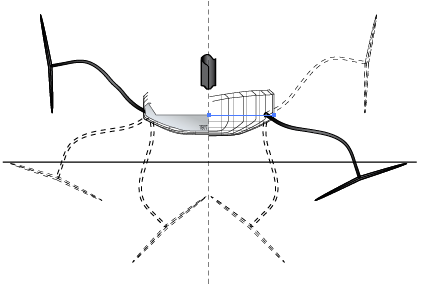
\includegraphics[height=26mm]{AC75-sketch.png}};
    \node[block, left of=plant, node distance=50mm] (actuator) {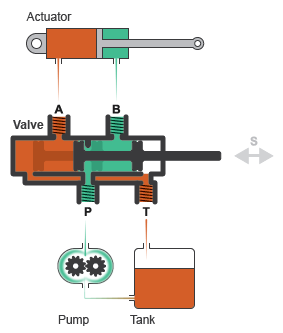
\includegraphics[height=40mm]{hydraulics.png}};
    \node[coordinate, left of=actuator, node distance=46mm, align=center] (controller) {
\includegraphics[width=16mm]{plc.png}\\Controlador};
    \node[coordinate, left of=controller, node distance=30mm] (input) {};
    \draw[->] ($ (controller.east) + (0, 0mm) $) -- node[above, align=left] {mueve\\ valvula} ($ (actuator.west) + (0, 0mm) $);
    \draw[->] (actuator) -- node[above] {fuerza} (plant);

  \end{tikzpicture}


\end{document}
